\documentclass[a4paper, 10pt]{article}
\usepackage[a4paper,left=3cm,right=2cm,top=2.5cm,bottom=2.5cm]{geometry}
\usepackage[utf8]{inputenc} % Change according your file encoding
\usepackage{graphicx}
%\usepackage[demo]{graphicx}
\usepackage{url}

\usepackage{float}
\usepackage{amsmath}
\usepackage{xcolor}
\usepackage{todonotes}

\usepackage{listings}

\definecolor{backcolour}{rgb}{0.95,0.95,0.92}

\lstdefinestyle{mystyle}{
    backgroundcolor=\color{backcolour},  
    breakatwhitespace=false,         
    basicstyle=\scriptsize,
    breaklines=true,                 
    captionpos=b,                    
    keepspaces=true,                 
    showspaces=false,                
    showstringspaces=false,
    showtabs=false,                  
    tabsize=2,
    frame=single
}



\lstset{style=mystyle}

%opening
\title{Seminar Report: Opty}
\author{\textbf{Ignacio Encinas Rubio, Adrián Jimenez González}}
\date{\normalsize\today{}}

\begin{document}

\maketitle

%\begin{center}
  %Upload your report in PDF format.
  
  %Use this LaTeX template to format the report.
  
	%A compressed file (.tar.gz) containing all your source code files must be submitted together with this report.
%\end{center}

\section{Introduction}


In this seminar we'll implement a transaction server using optimistic concurrency control with backwards validation. We'll study the behaviour of the transaction server under the variation of the different parameters to better understand it. Additionally, we have also explored some of its unintuitive behaviour and understood it. 

We have also carried out both lab extensions, comparing timestamp ordering with optimistic concurrency control while also implementing opty with forward validation.

\section{Code modifications}

   In this section we will briefly comment the code added to the template version in order to
   make the algorithm work. We will show the minimum number of lines of code possible to follow the reasoning.

  \subsection{Entry.erl}

    \begin{minipage}{.45\textwidth}
	\begin{lstlisting}[language=erlang, caption={Template}]
entry(Value, Time) ->
    receive
        {read, Ref, From} ->
            %% TODO: ADD SOME CODE
            entry(Value, Time);
        {write, New} ->
            entry(... , make_ref()); 
        {check, Ref, Readtime, From} ->
            if 
                 ... == ... ->  
                    %% TODO: ADD SOME CODE
                true ->
                    From ! {Ref, abort}
            end,
            entry(Value, Time);
        stop ->
            ok
    end.
 	\end{lstlisting}
    \end{minipage}\hfill
    \begin{minipage}{.45\textwidth}
	\begin{lstlisting}[language=erlang, caption={Filled version}]
entry(Value, Time) ->
    receive
        {read, Ref, From} ->
	    From ! {Ref, self(), Value, Time},
            entry(Value, Time);
        {write, New} ->
            entry(New , make_ref());
        {check, Ref, Readtime, From} ->
            if 
                 Readtime == Time -> 
		    From ! {Ref, ok};
                true ->
                    From ! {Ref, abort}
            end,
            entry(Value, Time);
        stop ->
            ok
    end.
  	\end{lstlisting}
  \end{minipage}

In this module we need to complete the \textbf{entry} function. This function is the responsible of the behaviour of the entries. The function will receive 3 types of message: read, write and check. 

\begin{itemize}
    \item  In case it receives a read message we will send a message with the \textit{Value}. The \textit{Ref} identifies the reading operation while \textit{Time} identifies the latest write performed in the entry and \textit{self()} the entry where it was performed.
  \item In case we receive a write message we will just update the \textit{Value} and obtain an identifier for it. 
  \item Finally, when we receive a check message, we must compare \textit{Readtime} of the message with our current timestamp, if it is the same we send an ok message (commit), else we send an abort message because the entry has been overwritten while we were performing our transaction.
\end{itemize}


\subsection{Handler.erl}

  \begin{minipage}{.45\textwidth}
	\begin{lstlisting}[language=erlang, caption={Template}]
handler(Client, Validator, Store, Reads, Writes) ->         
    receive
        {read, Ref, N} ->
            case lists:keyfind(..., ..., ...) of  %% TODO: COMPLETE
                {N, _, Value} ->
                    %% TODO: ADD SOME CODE
                    handler(Client, Validator, Store, Reads, Writes);
                false ->
                    %% TODO: ADD SOME CODE
                    %% TODO: ADD SOME CODE
                    handler(Client, Validator, Store, Reads, Writes)
            end;
        {Ref, Entry, Value, Time} ->
            %% TODO: ADD SOME CODE HERE AND COMPLETE NEXT LINE
            handler(Client, Validator, Store, [...|Reads], Writes);
        {write, N, Value} ->
            %% TODO: ADD SOME CODE HERE AND COMPLETE NEXT LINE
            Added = lists:keystore(N, 1, ..., {N, ..., ...}),
            handler(Client, Validator, Store, Reads, Added);
        {commit, Ref} ->
            %% TODO: ADD SOME CODE
        abort ->
            ok
    end.
 	\end{lstlisting}
    \end{minipage}\hfill
    \begin{minipage}{.45\textwidth}
	\begin{lstlisting}[language=erlang, caption={Filled version}]
handler(Client, Validator, Store, Reads, Writes) ->         
    receive
        {read, Ref, N} ->
            case lists:keyfind(N, 1, Writes) of  
                {N, _, Value} ->
		    Client ! {value, Ref, Value},
                    handler(Client, Validator, Store, Reads, Writes);
                false ->
		    Entry = store:lookup(N, Store),
		    Entry ! {read, Ref, self()},
                    handler(Client, Validator, Store, Reads, Writes)
            end;
        {Ref, Entry, Value, Time} ->
	    Client ! {value, Ref, Value},
            handler(Client, Validator, Store, [{Entry, Time}|Reads], Writes);
        {write, N, Value} ->
	    Entry = store:lookup(N, Store),
            NewWrites = lists:keystore(N, 1, Writes, {N, Entry, Value}),
            handler(Client, Validator, Store, Reads, NewWrites);
        {commit, Ref} ->
	    Validator ! {validate, Ref, Reads, Writes, Client};
        abort ->
            ok
    end.
  	\end{lstlisting}
  \end{minipage}

The next function we need to fill is on Handler module. The \textbf{handler} function expects to receive 4 types of messages: read, reply of entry, write and commit.

\begin{itemize}
    \item When we receive a read the first thing we have to do is check our list of writes. If we've written to that entry we know the value it will have. If not, we'll get the PID of the entry we have to read and forward the read message we've got from our client. 

  \item When we get the reply from the Entry we'll send the value to the Client and update the Reads list, as we will need it later in order to check for conflicts.
  \item If the message is a write, we look up for the entry and append or update the element in our Writes list. We'll need the number and Value\footnote{Both for the read bypass and the Value also when we commit the write}, the PID so that the validator can communicate with the entry.
  \item Last message we can receive is commit. With that message we need to send a validate message to the Validator with the whole state for our Client made of a Transaction ID (Ref, used to communicate an ok or an abort), the Reads, the Writes and the PID of the Client in order to communicate with it.
\end{itemize}

\clearpage
\subsection{Validator.erl}

In the validator module we have 3 functions to complete. 

\begin{minipage}{.45\textwidth}
	\begin{lstlisting}[language=erlang, caption={Template}]

validator() ->
    receive
        {validate, Ref, Reads, Writes, Client} ->
            Tag = make_ref(),
            send_read_checks(..., Tag),  %% TODO: COMPLETE
            case check_reads(..., Tag) of  %% TODO: COMPLETE
                ok ->
                    update(...),  %% TODO: COMPLETE
                    Client ! {Ref, ok};
                abort ->
                    %% TODO: ADD SOME CODE
            end,
            validator();
        stop ->
            ok;
        _Old ->
            validator()
    end.
 	\end{lstlisting}
    \end{minipage}\hfill
    \begin{minipage}{.45\textwidth}
	\begin{lstlisting}[language=erlang, caption={Filled version}]

validator() ->
    receive
        {validate, Ref, Reads, Writes, Client} ->
            Tag = make_ref(),
            send_read_checks(Reads, Tag),  
            case check_reads(length(Reads), Tag) of  
                ok ->
                    update(Writes),
                    Client ! {Ref, ok};
                abort ->
		    Client ! {Ref, abort}
            end,
            validator();
        stop ->
            ok;
        _Old ->
            validator()
    end.
  	\end{lstlisting}
  \end{minipage}


In the \textbf{validator} we wait for a request to validate a transaction. We do it by sending checking that none of our reads has been overwritten while we were doing the transaction. If we get no conflicts we'll make visible the Client's writes and send an ok message. In case of conflict we just send an abort message to the Client.


\begin{minipage}{.45\textwidth}
	\begin{lstlisting}[language=erlang, caption={Template}]

update(Writes) ->
    lists:foreach(fun({_, Entry, Value}) -> 
                  %% TODO: ADD SOME CODE
                  end, 
                  Writes).
 	\end{lstlisting}
    \end{minipage}\hfill
    \begin{minipage}{.45\textwidth}
	\begin{lstlisting}[language=erlang, caption={Filled version}]

update(Writes) ->
    lists:foreach(fun({_, Entry, Value}) -> 
		  Entry ! {write, Value}
                  end, 
                  Writes).
  	\end{lstlisting}
  \end{minipage}


  The next function to complete is \textbf{update}. We will call this function whenever we're sure our transaction is correct so we have to update the entries with their new values. To do so we'll just send the new value in a write message.


\begin{minipage}{.45\textwidth}
	\begin{lstlisting}[language=erlang, caption={Template}]
send_read_checks(Reads, Tag) ->
    Self = self(),
    lists:foreach(fun({Entry, Time}) -> 
                  %% TODO: ADD SOME CODE
                  end, 
                  Reads).
 	\end{lstlisting}
    \end{minipage}\hfill
    \begin{minipage}{.45\textwidth}
	\begin{lstlisting}[language=erlang, caption={Filled version}]

send_read_checks(Reads, Tag) ->
    Self = self(),
    lists:foreach(fun({Entry, Time}) -> 
		  Entry ! {check, Tag, Time, Self}
                  end, 
                  Reads).
  	\end{lstlisting}
  \end{minipage}

Last function is \textbf{send\_read\_checks}. We ask every entry we've read to confirm whether our previously read data has become stale or not. As we've covered before, this is done by checking if the write id has changed.

\clearpage

\subsection{Server.erl}

\begin{minipage}{.45\textwidth}
	\begin{lstlisting}[language=erlang, caption={Template}]
server(Validator, Store) ->
    receive 
        {open, Client} ->
            %% TODO: ADD SOME CODE
            server(Validator, Store);
        stop ->
            Validator ! stop,
            store:stop(Store)
    end.
 	\end{lstlisting}
    \end{minipage}\hfill
    \begin{minipage}{.45\textwidth}
	\begin{lstlisting}[language=erlang, caption={Filled version}]

server(Validator, Store) ->
    receive 
        {open, Client} ->
	    Client ! {transaction, Validator, Store},
            server(Validator, Store);
        stop ->
            Validator ! stop,
            store:stop(Store)
    end.
  	\end{lstlisting}
  \end{minipage}

  The last module we have to modify is \textbf{server}. From here we'll control the clients, sending them the Validator and Store that they will use.

\clearpage
\section{Performance}

We have used a shell script to automatize the testing and make the results easily reproducible. Every plot shows error bars for every point, but they are so small that they are not noticeable in most cases.

As indicated by the assignment we've tried to pick free parameters for each test in a way that lets us see the effect of the parameter under study. We've deviated a bit from the assignment and explored some peculiarities of the algorithm that came up from teacher suggestions. 

In the general case the algorithm performs very intuitively so result's discussion will not be too extensive. Keeping in mind that we're implementing and \textbf{optimistic} algorithm for concurrency control already hints us how it will behave under heavy contention. In addition to that, we have also read the paper discussing the design of Google's \textit{Omega}.

\subsection{Number of concurrent clients in the system}
\label{sec:numclients}

Increasing the number of clients makes it easier for them to clash, so it decreases the mean success rate pretty fast as can be seen in Figure \ref{fig:numclients}. Sections \ref{sec:magia} and \ref{timey-current-clients} give more information such as the limit for the success rate and the evolution for much higher number of clients respectively.


\begin{figure}[H]
  \centering
  \includegraphics[width=0.95\linewidth]{plots/numclients.pdf}
    \caption{Success rate w.r.t nº of clients}
    \label{fig:numclients}
\end{figure} 

In general, is safe to assume that if our number of concurrent client is not pretty small compared to the number of entries\footnote{Assuming uniform access among other things} opty is not a suitable option.



\clearpage
\subsection{Number of entries in the store}
\label{sec:numentries}
This is perhaps the most tricky parameter of our system. It shows extremely complex behaviour for some corner cases.

On the other hand, it is also true that our intuition holds for the majority of cases. That is, whenever $\text{entries} \gg \text{clients}$. Increasing the number of entries decreases the possibility of conflict, so it increases the success rate.
\begin{figure}[H]
  \centering
  \includegraphics[width=0.95\linewidth]{plots/numentries.pdf}
    \caption{Success rate w.r.t nº of entries}
    \label{fig:numentries}
\end{figure} 

\clearpage
\subsection{Number of reads per transaction}
\label{sec:numreads}
Doing more reads makes it easier for other clients to update those entries we've used and invalidate our transactions. It is so because of two reasons: we're increasing the number of different entries we read and the length of our transaction.

\begin{figure}[H]
  \centering
  \includegraphics[width=0.95\linewidth]{plots/numreads.pdf}
    \caption{Success rate w.r.t nº of reads}
    \label{fig:numreads}
\end{figure} 

\clearpage
\subsection{Number of writes per transaction}
\label{sec:numwrites}
Doing more writes increases the probability of updating an entry that had been previously read by other transaction that had not finished before we commited, so it decreases the success rate. It also makes our transaction take longer so the probability of our reads to be overwritten also grows.

\begin{figure}[H]
  \centering
  \includegraphics[width=0.95\linewidth]{plots/numwrites.pdf}
    \caption{Success rate w.r.t nº of writes}
    \label{fig:numwrites}
\end{figure} 


\clearpage
\subsection{Ratio of read/writes}
\label{sec:ratioreadwrites}

The conflicts appear whenever we read outdated data, so having very one sided transactions will result in almost no conflicts. The success rate decreases rapidly whenever we have a balanced transaction that performs both operations.

\begin{figure}[H]
  \centering
  \includegraphics[width=0.95\linewidth]{plots/ratio.pdf}
    \caption{Success rate w.r.t ratio of reads/writes with fixed amount of total operations}
    \label{fig:ratio}
\end{figure} 

Figure \ref{fig:ratio} shows that the behaviour is pretty simetric.

\clearpage

\subsection{Different percentage of accessed entries w.r.t the total number of entries}
\label{sec:nose}
A small percentage of accessed entries obviously increases our success rate, as the possibility for conflict is lower. It is also worth noting that this also introduces high variability on the success rate as some clients will access very crowded subsets while others will not.
\begin{figure}[H]
  \centering
  \includegraphics[width=0.95\linewidth]{plots/subset.pdf}
    \caption{Success rate w.r.t percentage of Entries accessible by each client}
    \label{fig:subset}
\end{figure} 


\subsection{What is the impact of each of these parameters on the success rate?}
Increasing the number of clients, reads and writes reduces the success rate, while increasing the number of entries increases it.

The results are very intuitive, because more complex transactions have higher probability of conflicting with others by reading entries that have been written.


On the other hand, there are some special cases where this intuition falls apart such as the one examined at Section \ref{sec:magia}. Results at Section \ref{sec:numentries} also indicate that adding entries can decrease the success rate for a low count of clients that perform complex transactions.


\subsection{Is the success rate the same for the different clients?}
In every plot we show the standard deviation via error bars. They're so small it's difficult to see them, so mainly yes. The only situation where the clients get different results is shown in Figure \ref{fig:subset}. It's expected as some clients will get subsets with very little \textit{traffic}, and other clients will compete with many others to access the same entries.

\clearpage
\subsection{Bonus. Minimum success rate per number of entries}
\label{sec:magia}
At first we can think that as we increase the number of clients the success rate will go to $0$. It's not such a wild idea but if we think carefully we'll notice that there is a pattern in our transactions that always succeeds: $\text{Write}_i \rightarrow \text{Read}_i \ | \ i \in [1, n]$. This gives us a lower bound on the amount of transactions that will succeed, as shown in Figure \ref{fig:magia}. In the simple case we've studied, in the $50\%$ of cases our transaction will be a write followed by a read. In order for it to succeed, the read will have to access the entry we've previously written, so the probability of doing so is $\frac{1}{n}$, where $n$ is the number of entries.

Obviously as the transaction complexity increases the calculation required to obtain this lower bound does too so we can't go much further, but surely anyone skilled enough in combinatorics could.
\begin{figure}[H]
  \centering
  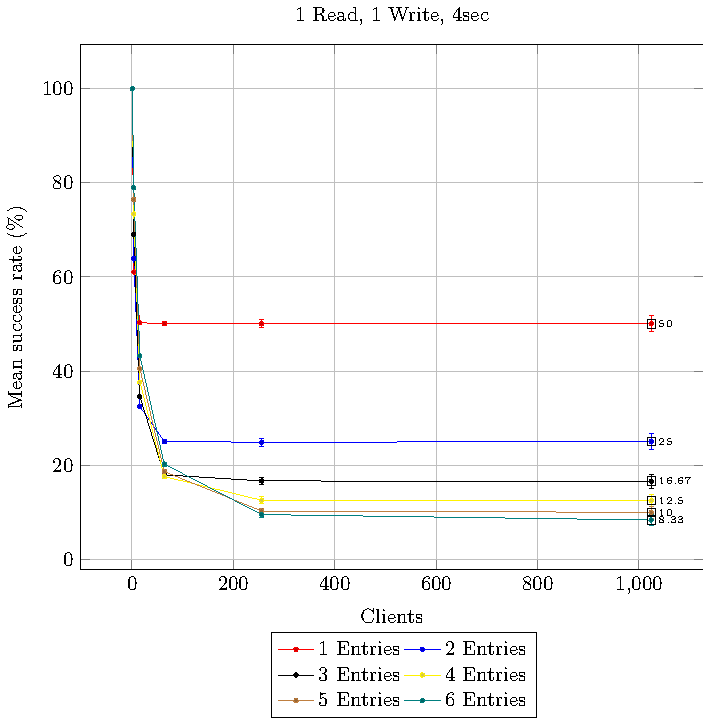
\includegraphics[width=0.90\linewidth]{plots/numentriesv2.pdf}
    \caption{Success rate w.r.t nº of clients and entries}
    \label{fig:magia}
\end{figure} 

This also helps explain the situation where adding entries does decrease the mean success rate\footnote{The case where it decreases for a low number of clients but complex transactions as in Figure \ref{fig:numentries} is yet to be understood}. It's very unintuitive but considering this lower bound makes it much more clear. When $\text{clients} \gg \text{entries}$ the conflicts will be unavoidable so the success rate will be very close to the lower bound, and increasing the number of entries decreases that lower bound significantly.

Obviously this is sort of a pathological example and it is not too representative. Surely the lower bound for any realistic transaction is so small that relying on this effect in order to sustain an acceptable lower bound makes no sense. Applying an algorithm for optimistic concurrency when you're expecting massive entry overload and contention would be pretty \textbf{bold}!

\clearpage

In order to check that our intuition is correct we've also checked with 2 Reads and 1 Write, where the expected lower bound would be $\displaystyle \frac{0.5}{n^2}$. The chance of starting the transaction with a write is still $50\%$ but now we have to hit the two consecutive reads in the same entry we read, thus getting a probability of $0.5 \cdot \frac{1}{n} \cdot \frac{1}{n}$. Figure \ref{fig:magia2} illustrates the expected trend. Similarly, we have replicated the results for other simple configurations.
\begin{figure}[H]
  \centering
  \includegraphics[width=0.95\linewidth]{plots/numclients2.pdf}
    \caption{Success rate w.r.t nº of clients and entries}
    \label{fig:magia2}
\end{figure} 

Overall, noticing this effect after discussing it in the labs session has been very enjoyable. Of course it is not of any practical use as we've already mentioned, but it shows how complex distributed systems are.

\clearpage
\section{Distributed execution}

For this experiment, we have made a few changes to generate a process in another node from one unique start function. The changes have been done in the \textit{opty} module. 

To be able to call the distributed server we have to register it and have it on the client side. We have used the piece of code from listing \ref{list:register}.


\begin{minipage}{\textwidth}
  \begin{lstlisting}[language=erlang, caption={Register Distributed Server}, label={list:register}]
    spawn(Snode, fun() -> 
                         register(s, server:start(Entries))end),
  
 	\end{lstlisting}
\end{minipage}

Figures \ref{fig:2nodes}-\ref{fig:1node} it is shown the execution of the distributed algorithm. In the first one, we can see two nodes, in which we run clientside and serverside. In the right terminal, it is shown that \texttt{s} is created in the server node and the start function is executed in the client node (left terminal). 

Also, to show the correct behaviour, in figure \ref{fig:1node}, the server node is down and we can not spawn the server in that node, so the algorithm does not work.


When we run \textit{Opty} in a Distributed Erlang, the handler is in the client node.



\begin{figure}[H]
  \centering
  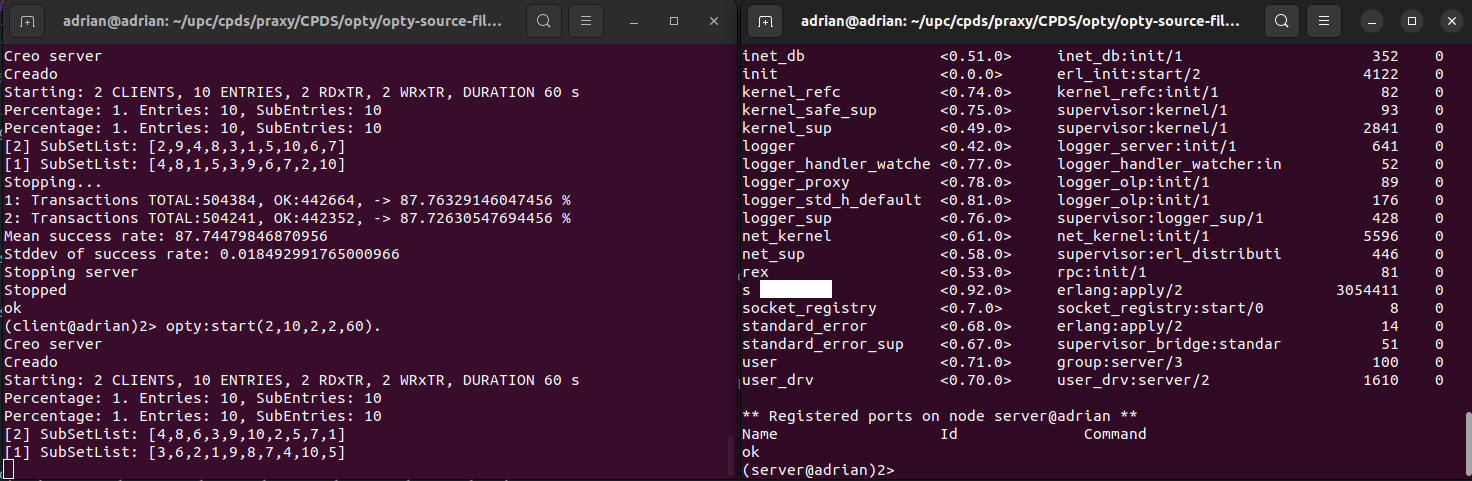
\includegraphics[width=0.95\linewidth]{images/optyWorking.png}
    \caption{Opty working in 2 nodes}
    \label{fig:2nodes}
\end{figure} 


\begin{figure}[H]
  \centering
  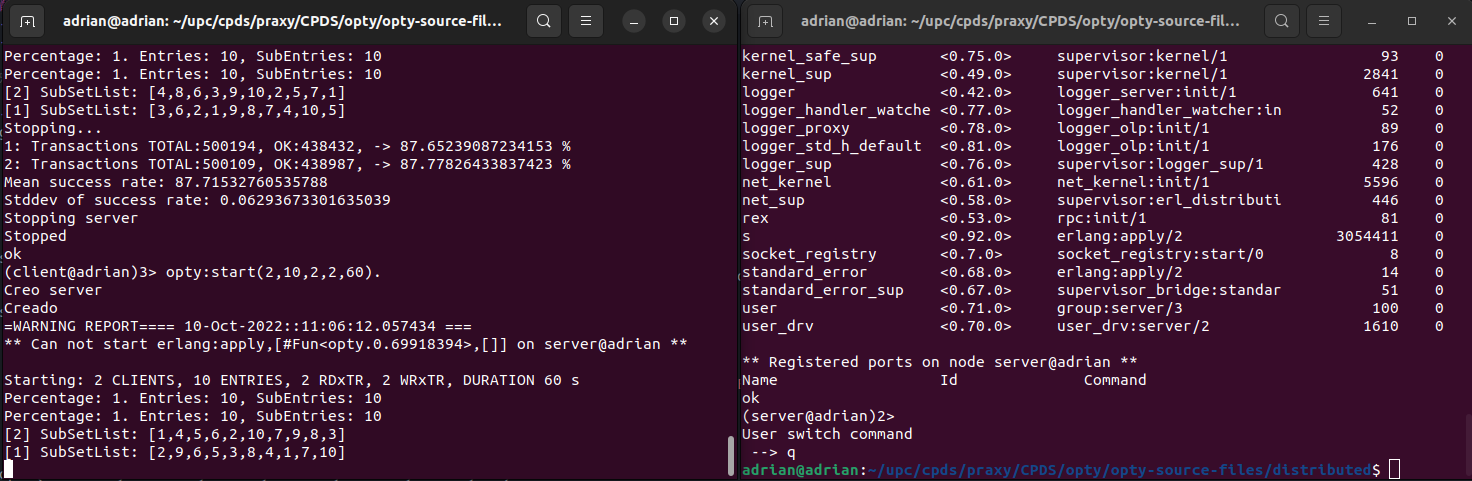
\includegraphics[width=0.95\linewidth]{images/opty1node.png}
    \caption{Opty failing with 1 node}
    \label{fig:1node}
\end{figure} 

\clearpage
\section{Other concurrency control techniques}

In this section we'll compare timestamp ordering with optimistic concurrency control. We've tried to be exhaustive but sadly there are some results left to be understood such as the ones shown at Figure \ref{timey:subset}\footnote{Here we're specifically talking about the brown line. We discussed and explored possible causes such as imbalance in the subset distributions and so on but we couldn't come up with a satisfactory explanation}.

There are some notable differences among both approaches. In \textit{Timey} we'll know whether or not our transaction will succeed after every entry involved has been informed of our operations, but we'll have to wait\footnote{Generally speaking, of course we have read-bypass for our own writes} for a response. On the other hand, \textit{Opty} offers us more responsiveness at the cost of making us do useless work in some cases. Timestamp ordering also introduces a new type of conflicts: Write $\rightarrow$ Write. If $\text{Write}_{t_2}$ is processed before $\text{Write}_{t_1}$ (with $t_1 < t_2$) we'll have to reject $\text{Write}_{t_1}$. Timey's extensive bookeeping also allows us to tolerate concurrent Reads and Writes, as we'll apply them in an ordered manner whenever possible.

Even though we're only considering success rates we think that other differences such as the latencies and tolerance to overload are very important when considering this algorithms in a real scenario.

\subsection{Number of concurrent clients in the system}\label{timey-current-clients}

As we mentioned in Section \ref{sec:numclients}, in optimistic control, increasing the number of clients makes clashes more frequent, reducing the success ratio. When we increase the number of clients with timestamp control (timey), the number of clients also reduces the success ratio, but not that drastically, as it is shown in Figure \ref{timey:numclients}. 

In the \textit{timey} algorithm, temptative reads and writes are allocated in an queue ordered by the timestamp, discarding only the transactions that don't satisfy the consistency checks. In the case of writes the timestamp must be higher than the last write's timestamp and greater or equal than the latest read timestamp. For read operations we just have to check that it's timestamp is higher than the last write.

\begin{figure}[H]
  \centering
  \includegraphics[width=0.75\linewidth]{timey_plots/numclients2.pdf}
    \caption{Success rate w.r.t nº of clients}
    \label{timey:numclients}
\end{figure} 

Figure \ref{timey:numclients} indicates that there are also interesting patterns in \textit{Timey} such as hard lower bounds depending on the parameters of the system.

\clearpage
\subsection{Number of entries in the store}

The results show us that the bigger the number of entries for the number of clients, the best the success rate we obtain for both algorithms. Both \textit{Timey} and \textit{Opty} show similar evolution, although \textit{Opty} is more sensible to small entry counts because the number of conflicts spikes. 

\begin{figure}[H]
  \centering
  \includegraphics[width=0.95\linewidth]{timey_plots/numentries.pdf}
    \caption{Success rate w.r.t nº of entries}
    \label{timey:numentries}
\end{figure} 

Figure \ref{timey:numentries} shows that \textit{Timey} can tolerate a smaller number of entries. This is intuitive because \textit{Timey} is designed to deal with conflicts, while \textit{Opty} assumes a small number of them and optimizes for quick response times.


\clearpage
\subsection{Number of reads per transaction}
\label{timey_sec:numreads}

Doing more reads per transaction decreases the success rate for \textit{Opty} significantly. \textit{Timey} is able to sustain a much higher success rate as shown in Figure \ref{timey:numreads}. This makes sense because \textit{Timey} will keep a list of pending operations and apply them in an ordered manner, and this allows us to tolerate concurrent reads and writes for a small number of writes.

\begin{figure}[H]
  \centering
  \includegraphics[width=0.95\linewidth]{timey_plots/numreads.pdf}
    \caption{Success rate w.r.t nº of reads}
    \label{timey:numreads}
\end{figure} 

\clearpage
\subsection{Number of writes per transaction}
\label{timey_sec:numwrites}

Doing more writes per transaction decreases the success rate in both algorithms in a similar way. Figures \ref{timey:numwrites} and \ref{timey:ratio} show that \textit{Timey} can perform worse than \textit{Opty} for very write-intensive transactions. It makes sense as Write $\rightarrow$ Write conflicts are possible now.

\begin{figure}[H]
  \centering
  \includegraphics[width=0.95\linewidth]{timey_plots/numwrites.pdf}
    \caption{Success rate w.r.t nº of writes}
    \label{timey:numwrites}
\end{figure} 

\clearpage
\subsection{Ratio of read/writes}

\textit{Timey} shows somewhat similar behaviour with respect to \textit{Opty} but performing notably better for read-intensive transactions and a bit worse for write-intensive transactions. This is expected following the conclusions reached at Sections \ref{timey_sec:numreads} and \ref{timey_sec:numwrites}. It is worth noting that \textit{Timey} doesn't get 100\% success rate for write-only transactions as the Write $\rightarrow$ Write conflict is possible.


\begin{figure}[H]
  \centering
  \includegraphics[width=0.95\linewidth]{timey_plots/ratio.pdf}
    \caption{Success rate w.r.t ratio of reads/writes with fixed amount of total operations}
    \label{timey:ratio}
\end{figure} 

\clearpage
\subsection{Different percentage of accessed entries w.r.t the total number of entries}

Our intuition tells us that increasing the percentage of accessed entries will decrease the success rate as the possibility of conflicting with other clients is higher. This effect can be seen at some test cases in Figure \ref{timey:subset} for both algorithms, although \textit{Timey} shows less variation. We have also encountered a weird case for \textit{Timey} when increasing the number of accessed entries increases the success rate. We have not been able to come up with a satisfactory explanation for this effect.


\begin{figure}[H]
  \centering
  \includegraphics[width=0.95\linewidth]{timey_plots/subset.pdf}
    \caption{Success rate w.r.t percentage of Entries accessible by each client}
    \label{timey:subset}
\end{figure} 


We can conclude that timestamp ordering is more versatile than optimistic concurrency control as expected. Success rates are notably higher in the majority of cases and won't let clients make useless work. It is also true that \textit{Opty} can offer better latencies and could be more suitable for workloads with not many conflicts.

\clearpage


\section{Forward validation}

To implement \textbf{forward validation} we need to modify the source code of some modules. These modules are handler, validator and entry. Validator and entry have the most changes to modify the behaviour of the checking phase. Meanwhile, handler only needs minor changes to match the structure of new messages to send to the validator and entries.

\subsection{Entry}

In this module, we have introduced a series of changes to accomplish forward validation. First of all, now we do not need to check when \textit{read} messages arrive. The validator will need to compare its Write list with the Reading list of the Entry. For that, we are going to implement a Reading list in Entry module, in which we will add the PID of the Handler every time it read (this implementation will need to take care of deleting all the appearances of that handler, discussed below).

With this change in \textit{read} messages, the behaviour on \textit{write} messages changes. Now, this kind of messages do not need to validate anything, so they will update directly.

\textit{Check} messages have the bigger change. They will change not only the structure but also all their behaviour. Now we check if the list of Reads is empty, which means that no one had read that entry so we are able to commit our transaction. Otherwise, we abort the transaction if there are some PID in our Read list. We are checking if there is an empty list because before checking validator asks for the entry for deleting the PID of the handler of the transaction.

Also, we will need \textit{block} and \textit{unblock} messages to block/unblock the entry while Validator is validating.

The last type of message is \textit{delete}. This message deletes every occurrence of the requested PID from the Read list from the entry.

\subsection{Validator}

The validator module needed a few changes in addition to the new entry messages structure. We are introducing some functions like ``send\_write\_check'' and ``check\_writes'', are responsible for sending check messages to the corresponding entries and receiving their answers to complete or abort the transactions.

Inside of \texttt{validator} function, we are waiting for a \textit{validate} message from the handler. The first thing we have to do is to block every entry we've written to and deleting every occurrence of the handler's PID from ALL the entries he is attempting to write. Then, it sends the checks messages with the previous functions, and depending on the response (ok or abort), it will update the Writes and finish the transaction successfully or abort it. After these actions, the validator will need to delete also the Reads of that transaction in the corresponding entries in which the handler has read. Finnaly, it will unblock the entries that we blocked before.


\subsection{Handler}

As mentioned before, this module only had some minor changes. They are focused on following the structure of the changed messages.

\clearpage

\subsection{Message Diagram}

To clarify the messages introduces, a diagram has been created. In figure \ref{fig:diagram} we can see the messages we are passing between the three modules we made changes and their structures.

\begin{figure}[H]
  \centering
  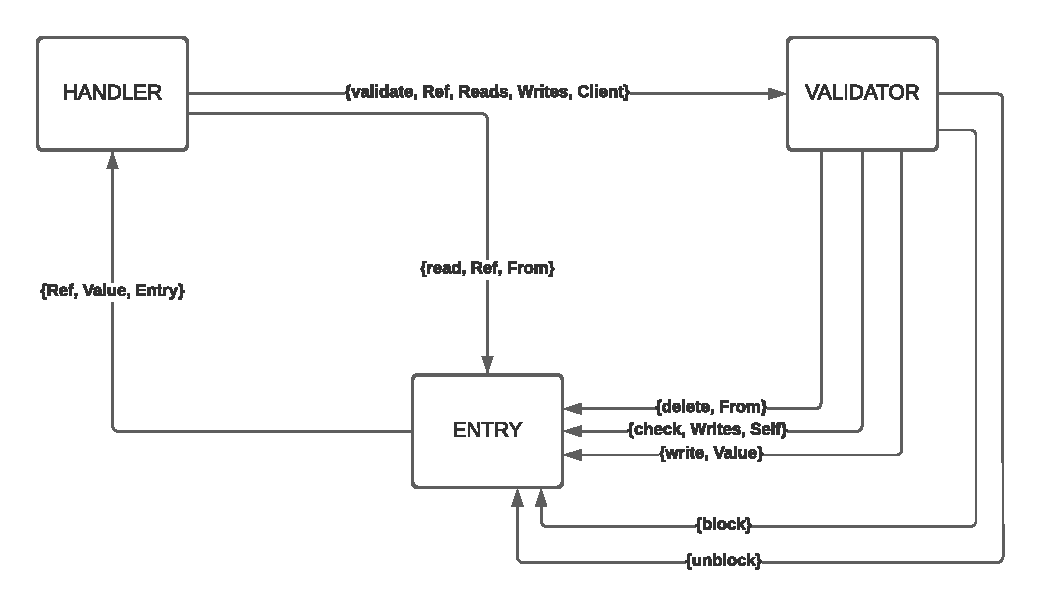
\includegraphics[width=0.95\linewidth]{images/messagesForward.pdf}
    \caption{Message diagram of Opty with Forward Validation}
    \label{fig:diagram}
\end{figure} 

\clearpage

\subsection{Comparison with respect to Backward Validation}
In order to check whether our implementation is working as expected or not, we've obtained some results that we'll compare the previous ones. 

Regarding the obtained results, they are as expected as our clarifications with the teacher. They show that forward validation performance is lower than backward validation in almost all test we tried. Just in the experiment in which we increase the number of writes per transaction, we obtain better results than backward validation.

In all the figures we show below we have taken the results for backward validation, forward validation, and forward validation without entry blocking\footnote{As we already obtained results for this incorrect implementation, we thought it would be nice to see the effects in the common plots}.


\begin{figure}[H]
  \centering
  \includegraphics[width=0.95\linewidth]{forward/ratio.pdf}
    \caption{Success rate w.r.t ratio of read/writes with fixed amount of total operations}
    \label{}
\end{figure} 

\begin{figure}[H]
  \centering
  \includegraphics[width=0.95\linewidth]{forward/numclients.pdf}
    \caption{Success rate w.r.t nº of clients}
    \label{}
\end{figure} 

\begin{figure}[H]
  \centering
  \includegraphics[width=0.95\linewidth]{forward/numreads.pdf}
    \caption{Success rate w.r.t. nº of reads}
    \label{}
\end{figure} 

\begin{figure}[H]
  \centering
  \includegraphics[width=0.95\linewidth]{forward/numwrites.pdf}
    \caption{Success rate w.r.t nº of writes}
    \label{}
\end{figure} 

%numclients.pdf
%numreads.pdf
%numwrites.pdf
%ratio.pdf


\clearpage
\section{Personal opinion}

\subsection{Ignacio}

The assignment has been interesting. Specially, trying to understand the weird corner cases. Perhaps adding delays in the Clients to fake the work they're doing and compare the different latencies for the algorithms could be a good extension.

\subsection{Adrián}

In my opinion this practice have been interesting. I learned a bit more of Erlang and taking some challenges that previous practice didn't have. We have understand the opty algorithm and also timey to compare them. Also the main challenge (from my point of view) of modify the opty code without a "guide" code to implement forward validation, truly facing with Erlang language.

\end{document}
